\section{W01 - Operations Management}
 
\subsection{Introduction to OPM}
\subsubsection{What is Operations (and Process) Management?}
Operations and process management is the activites of managing the resources that produce products and services. 
Soll heissen:
Leistung erstellen, Produktion \& Logistik, F\"uhren \& lenken der Ressourcen
\subsubsection{Why Is w.1OP Highly Relevant for the Banking, Finance, and Insurance Industries?}
Industrialization as a Megatrend in Services
\subsubsection{IKEA’s Success Factors}
\begin{center}
	\begin{tabular}{|c|l|}
		\hline	3 Hauptprozesse\index{3 Hauptprozesse} in einem Unternehmen&\\
		\hline \multirow{2}{*}{Leistungserstellung}   & G\"unstig = tiefe Kosten \\
		(Operation = Gewinn) &Economics of scale = Hohes Volumen, konzentration \\
		& der Fertigung (\index{SCM}SCM) \\
		 
		\hline \multirow{5}{*}{Innovationsprozesse} & Produktekonzept \\ 
		& * Kunde baut zusammen \\
		& * Kunde holt aus Lager  \\
		& * Produktionskonzept \\
		& * Service design \\
		\hline \multirow{3}{*}{Marketing, Verkauf/Kundenprozess} & Verkaufskonzept \\ 
		& Standort \\
		& Erlebnis \\
		\hline 
	\end{tabular} 
\end{center}
\subsection{Core Activities}
\subsubsection{Where Does a Business Get Its Competitive Edge?}
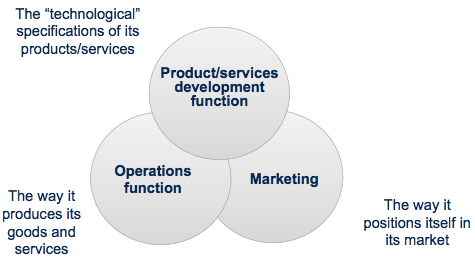
\includegraphics[width=1\textwidth]{W01/competitive_edge}
\subsubsection{Operations Can be Analyzed at Three Levels}
\index{Operations!Levels}
\index{Flow between! operations}
\index{Flow between! processes}
\index{Flow between! resources}
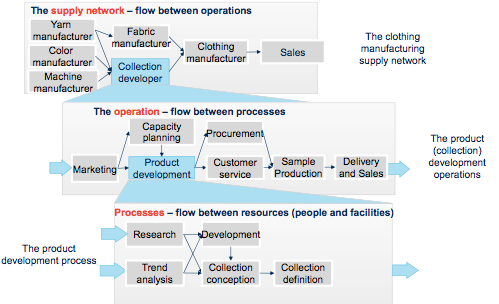
\includegraphics[width=1\textwidth]{W01/operations_three_levels}
\subsubsection{The Output of Most Types of Operation: A Mixture of Goods and Services}
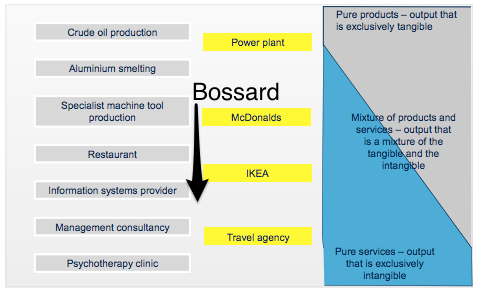
\includegraphics[width=1\textwidth]{W01/goods_and_services}
Bossard group bietet Verbindungstechnik als Dienstleistung. (Mixture  \index{Products}Products and \index{Service}Service)
\index{Pure!Products} \index{Pure!Services}
\subsubsection{Core and Supporting Processes/Functions }
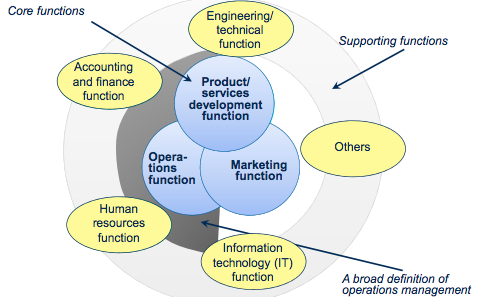
\includegraphics[width=1\textwidth]{W01/core_and_supporting_processes}
\index{Functions!Core}
\index{Functions!Supporting}

\subsection{Characteristics of OPM}
\subsubsection{Differences Within Sectors Are often Greater than the Differences between Sectors}
Aufgepasst beim Vergleich mit Branchenkennzahlen!\\
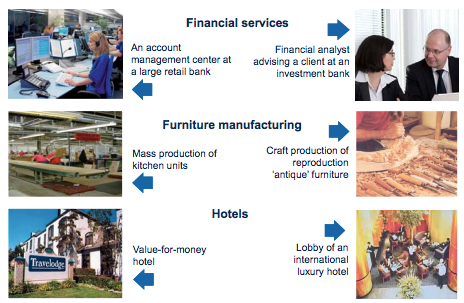
\includegraphics[width=1\textwidth]{W01/differences_betwee_sectors}
\subsubsection{The Four V’s: The Typology of Operations}
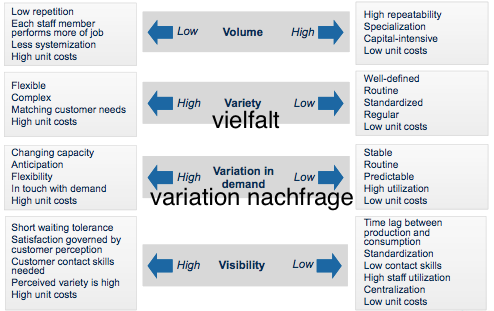
\includegraphics[width=1\textwidth]{W01/four_v}
\index{4V!Volume}
\index{4V!Variety}
\index{4V!Variation in Demand}
\index{4V!Visibility}
\subsubsection{Profiles of Different Types of Restaurants (4V)}
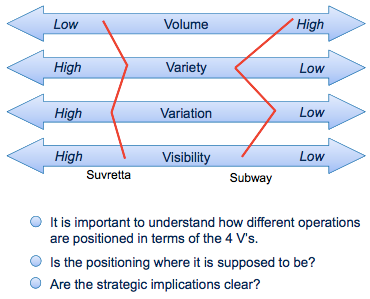
\includegraphics[width=1\textwidth]{W01/4v_restaurant}






